% ====================================================================
%  Self-contained source: preamble and body merged.
%  Generated by flatten.py -- edit manuscript_zh.md and rerun
%  build_zh.sh, not this file.
%  Compile with xelatex, twice.  Figures are expected in ../figures/;
%  for arXiv, copy them alongside and set \graphicspath{{./}}.
%  arXiv does not run BibTeX: submit main.bbl with this file.
% ====================================================================

\documentclass[11pt,a4paper]{article}
\usepackage[margin=2.4cm]{geometry}
\usepackage{amsmath,amssymb}
\usepackage{graphicx}
\usepackage{booktabs}
\usepackage{longtable}
\usepackage{array}
\usepackage{caption}
\usepackage[table]{xcolor}
\usepackage[colorlinks=true,linkcolor=black,citecolor=black,urlcolor=blue]{hyperref}
\usepackage[numbers,sort&compress,square]{natbib}
\bibliographystyle{unsrtnat}
\usepackage{enumitem}
\setlist{nosep,leftmargin=1.6em}

\usepackage{fontspec}
\usepackage{xeCJK}
\setmainfont{DejaVu Serif}[Scale=0.92]
\setsansfont{DejaVu Sans}[Scale=0.9]
\setmonofont{DejaVu Sans Mono}[Scale=0.85]
\setCJKmainfont{Noto Serif CJK SC}
\setCJKsansfont{Noto Sans CJK SC}
\setCJKmonofont{Noto Sans Mono CJK SC}
\usepackage{unicode-math}
\setmathfont{DejaVu Math TeX Gyre}

% Chinese typographic conventions
\XeTeXlinebreaklocale "zh"
\XeTeXlinebreakskip = 0pt plus 1pt minus 0.1pt
\linespread{1.25}
\setlength{\parindent}{2em}

\captionsetup{font=small,labelfont=bf,width=0.92\textwidth}
\renewcommand{\figurename}{图}
\renewcommand{\tablename}{表}
\renewcommand{\refname}{参考文献}
\renewcommand{\bibname}{参考文献}
\graphicspath{{../figures/}}

\providecommand{\tightlist}{%
  \setlength{\itemsep}{0pt}\setlength{\parskip}{0pt}}
\providecommand{\pandocbounded}[1]{#1}

\title{\bfseries 弹性尺寸失配的物理上限：\\
统计无序能否导致 bcc 钽的固溶软化？\\[6pt]
\large Ta(Lu) 体系的扭折对动力学蒙特卡洛研究\\
及一项预先设定判据的第一性原理检验}
\author{吴荣华\thanks{珠海九重天航空科技有限公司，中国珠海。
\texttt{wrh@gdtzn.com}}
\and 陈儒庆\thanks{GUT Geoservice Inc.，加拿大蒙特利尔。
\texttt{ruqing@hotmail.com}}}
\date{\number\year 年 \number\month 月 \number\day 日}

\begin{document}
\maketitle


\hypertarget{ux6458ux8981}{%
\section*{摘要}\label{sec:ux6458ux8981}}

bcc 金属中的固溶软化通常被归因于溶质对扭折对形核的影响，但弹性无序与直接的核心化学效应二者的相对权重从未被定量分离。本文以 Ta(Lu) 作为上限探针来处理这一问题。该体系在冶金学上不可实现------Lu 在 Ta 中的平衡固溶度低于 0.1 at.\%，且不存在任何中间化合物------但其 18.5\% 的线性失配与 11.4 ų 的弛豫体积，使弹性尺寸相互作用达到了难熔基体中所能达到的上限。由于涨落软化项按相互作用强度的平方标度，而与之竞争的硬化通道按一次方标度，本体系代表了弹性无序所能呈现的最有利情形，因而一个否定性结果可以外推到更弱的溶质体系。

综合运用各向异性 Stroh 场------我们证明它使 \(\tfrac12\langle111\rangle\) 螺型位错获得一个 \(\cos3\theta/r\) 的体胀场，而该场在通常的各向同性假设下严格为零------半巨正则系综的溶质气团采样，以及扭折对动力学蒙特卡洛，我们发现：在 100 至 450 K 的全部温区内，随机 Lu 溶质场都\textbf{提高}了速率控制型 \(\tfrac12\langle111\rangle\) 螺位错的流变应力。涨落诱导的势垒降低在 100 K 时达到 85 meV，为纯金属形核焓的 9.4\%，但被扭折迁移阻力以及形核鞍点的极值取样偏置所压倒；后者部分源自离散化模型本身，我们保留它作为一种保守选择。

引入唯象的化学软化项后，只有当其超过 150 K 下的 \(\kappa^* = 0.17 \pm 0.03\) eV（即纯金属扭折对焓的 19\%）时符号才发生反转，且在约 250 K 以上任何 \(\kappa\) 值都无法产生软化。我们将 \(\kappa^*\) 作为第一性原理核心计算的可证伪阈值提出，同时指出它是相对于一个占位符核心结合能定义的，必须与之同步重新计算。

\begin{center}\rule{0.5\linewidth}{0.5pt}\end{center}

\hypertarget{ux5f15ux8a00}{%
\section{引言}\label{sec:ux5f15ux8a00}}

向金属中加入溶质通常会提高其流变应力。但在 bcc 金属中，当温度低于约 \(0.2\,T_m\) 时，有时会观察到相反的现象：W(Re)、Mo(Re) 与 Fe(Si) 都会先软化，而后在更高温度下硬化 \cite{christian1983}。这一效应具有技术意义------它是难熔金属韧化的途径之一------而其成因在六十年间始终未有定论。

bcc 金属的低温塑性由 \(\tfrac12\langle111\rangle\) 螺型位错控制 \cite{hirth1982,dezerald2014}。其紧致的非平面核心赋予它很高的 Peierls 应力，滑移机制则依赖热激活的扭折对形核。因此软化必然作用于这一机制，而通常有两条途径被提出：

\textbf{（M1）统计机制。} 随机溶质场使扭折对形核势垒成为一个随机变量。形核会取样其分布的低尾部，因此对方差为 \(\sigma^2\) 的高斯型势垒分布，有效激活焓被降低 \(\sigma^2/2k_BT\) \cite{labusch1970,kocks1975}。该项随温度降低而增大，因此仅凭无序本身------不需要任何化学效应------原则上就能在低温使 bcc 金属软化。

\textbf{（M2）化学机制。} 溶质在电子层面改变位错核心，直接降低 Peierls 势垒本身。这超出了连续介质弹性力学的范畴。

观察到软化并不能区分这两者：二者预言的符号相同，温度依赖也相似。区分它们的方式是追问 M1 是否\textbf{充分}------而这个问题具有清晰的计算形式，因为 M1 完全由可精确计算的弹性量决定。

本文在 M1 最强的位置上提出这一问题。我们在弹性尺寸效应的物理上限处构建溶质--位错模型，通过原子尺度与介观尺度模拟向上传递，并检验软化是否出现。结果是没有出现。随后我们定量化学机制必须提供多少------一个严格相对于所假设的核心结合能而定义、必须与之同步重算的阈值 \(\kappa^*\)------并将该数值预注册为第一性原理计算的检验目标。

\begin{center}\rule{0.5\linewidth}{0.5pt}\end{center}

\hypertarget{ux4e3aux4f55ux9009ux62e9-talu}{%
\section{为何选择 Ta(Lu)}\label{sec:ux4e3aux4f55ux9009ux62e9-talu}}

Ta(Lu) 并非候选结构合金。Lu 在 Ta 中的平衡固溶度低于 0.1 at.\%，不存在中间化合物，其相关的实验情境是通过分子束外延或磁控溅射在远离平衡的条件下生长的过饱和薄膜。我们有意采用该体系，且这一选择在论证中承担实质作用，而非可有可无。

取 \(r_{\rm Lu} = 1.73\) Å 与 \(r_{\rm Ta} = 1.46\) Å，线性失配为 18.5\%，是任何难熔基体中所能得到的最大值之一。由实测原子体积给出弛豫体积：

\[\Omega_{\mathrm{Ta}} = a_0^3/2 = 18.07\ \text{\AA}^3,\qquad \Omega_{\mathrm{Lu}} = \tfrac{\sqrt{3}}{4}a^2c = 29.5\ \text{\AA}^3 \;\Longrightarrow\; \Delta V = 11.45\ \text{\AA}^3,\]

与硬球估计 \(\Omega_{\mathrm{Ta}}[(1+\varepsilon)^3-1] = 12.0\) ų 相差 5\% 以内。注意线性化式 \(\Delta V \simeq 3\Omega\varepsilon\) 仅在 \(\varepsilon\) 很小时成立，此处将给出 0.555 而非 0.664，即 \$\sim\$20\% 的误差，传递到临界应力上约为 25\%。

标度论证使这一极端失配成为必需：

\begin{itemize}
\tightlist
\item
  M1 的软化项按 \(\sigma^2/2k_BT\) 标度，即按 \(U^2\) 标度，其中 \(U\) 为溶质--位错相互作用强度；
\item
  与之竞争的硬化通道------扭折迁移阻力与形核鞍点的极值取样偏置------按 \(U\) 标度。
\end{itemize}

因此软化与硬化之比\textbf{随失配线性增长}。Ta(Lu) 是 M1 在 bcc 基体中所能呈现的最有利情形。否定性结果可外推至更弱的溶质，而不局限于本体系。我们事先声明：肯定性结果不具备这一性质，届时将作为体系特定的结论报告。

\begin{center}\rule{0.5\linewidth}{0.5pt}\end{center}

\begin{figure}[htbp]\centering
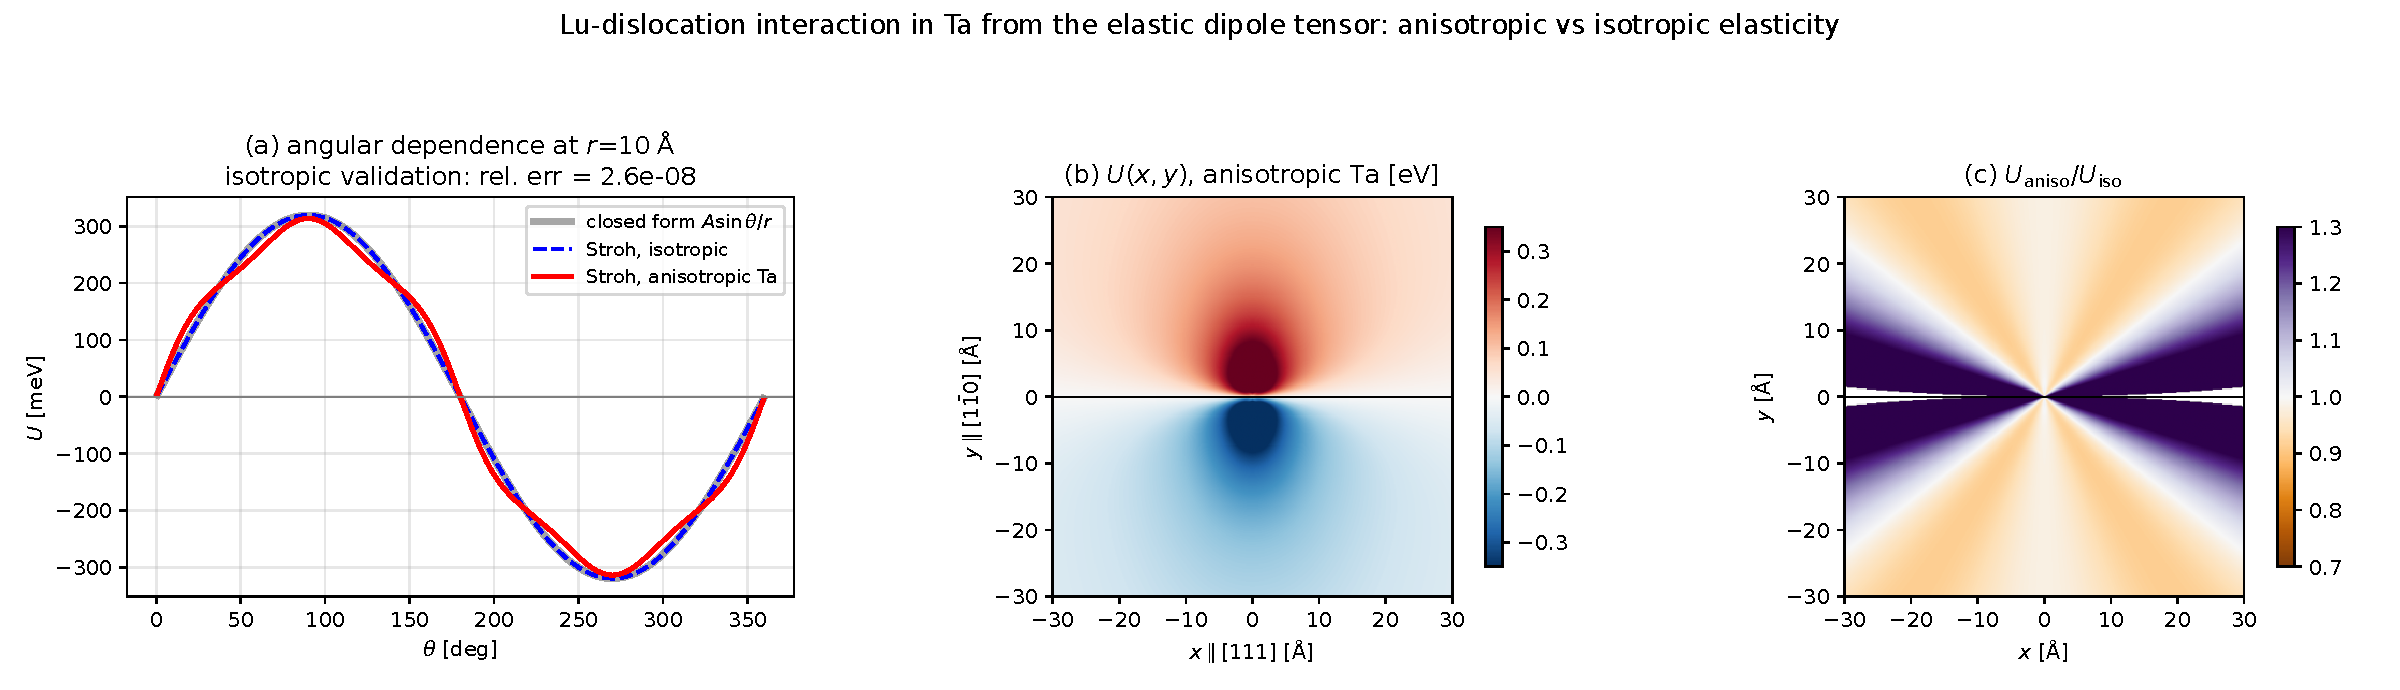
\includegraphics[width=1.0\linewidth]{fig1_elastic_fields.pdf}
\caption{由弹性偶极张量给出的溶质--位错相互作用。(a) $r=10$\,\AA\ 处的角向依赖；各向同性 Stroh 解复现闭式解 $A\sin\theta/r$，误差 $2.6\times10^{-8}$。(b) 刃型位错的各向异性场。(c) 各向异性与各向同性之比：振幅仅变化 $-1.8\%$，但在滑移面附近角向形状偏差达 $\pm30\%$，而那正是 $\mathrm{d}U/\mathrm{d}x$ 控制钉扎的区域。}
\label{fig:fig1}
\end{figure}

\hypertarget{ux65b9ux6cd5}{%
\section{方法}\label{sec:ux65b9ux6cd5}}

\hypertarget{ux5f39ux6027ux573a}{%
\subsection{弹性场}\label{sec:ux5f39ux6027ux573a}}

溶质--位错相互作用由弹性偶极张量计算：

\[U(r,\theta) = -P_{ij}\,\varepsilon_{ij}^{\rm disl}(r,\theta),\]

位错应变场取自各向异性 Stroh 六次型形式 \cite{stroh1958,hirth1982}，采用 Clouet 等的弹性偶极框架 \cite{clouet2018} 与 Ta 的弹性常数 \cite{featherston1963} \(C_{11}/C_{12}/C_{44} = 266.0/158.2/87.4\) GPa（Zener 各向异性 \(A = 1.622\)，\(K = 194.1\) GPa）。

\textbf{一条约束整个处理的对称性结果。} 占据 bcc 格点的置换式溶质具有完整的 \(O_h\) 位点点群。在 \(O_h\) 下不变的对称二阶张量必须是各向同性的，故

\[\boxed{P_{ij} = P\,\delta_{ij}\ \text{（严格成立）}},\qquad P = K\,\Omega_{\rm rel} = 13.87\ \text{eV},\]

\textbf{与失配大小无关}。置换式溶质在立方基体中不存在一阶四方畸变，也不存在 Fleischer 剪切耦合。剪切耦合只能通过介弹极化率 \(\alpha_{ijkl} = -\partial P_{ij}/\partial\varepsilon_{kl}\) 在二阶出现 \cite{fleischer1962,clouet2018}。这正是它与间隙式溶质（如 bcc 铁中的碳）的定性差别：后者的八面体位点对称性给出四方偶极张量与很大的一阶剪切耦合。

因此只有体胀分量 \(\varepsilon_{kk}\) 进入，相互作用简化为 \(U = -P\varepsilon_{kk}\)。

程序实现已对照各向同性闭式解 \(U = A\sin\theta/r\)（其中 \(A = (1+\nu)\mu b\Delta V/[3\pi(1-\nu)] = 3.196\) eV\(\cdot\)Å）验证，最大相对误差 \(2.6\times10^{-8}\)。

核心正则化采用光滑形式

\[U = \frac{A\,r\sin\theta}{r^2 + r_c^2},\qquad r_c = \frac{A}{2U_{\rm cap}},\]

它在 \(r \gg r_c\) 时回到远场解，在核心处平滑趋零，峰值恰为 \(U_{\rm cap}\)。若改用硬截断，则在 \(U(x)\) 中引入约 0.4 eV 的阶跃，其数值导数是高度 \(\propto1/dx\)、宽度 \(\propto dx\) 的力尖峰；我们发现这会使临界应力随网格间距漂移 57\%，且非单调（见 5.1 节）。

线张力采用 de Wit--Koehler 取向依赖关系 \cite{dewit1959} \(\Gamma = E + d^2E/d\theta^2\)：

\[\Gamma_{\rm edge} = \frac{\mu b^2(1-2\nu)}{4\pi(1-\nu)}\ln\frac{R}{r_0} = 0.940\ \text{eV/\AA},\qquad \Gamma_{\rm screw} = \frac{\mu b^2(1+\nu)}{4\pi(1-\nu)}\ln\frac{R}{r_0} = 3.935\ \text{eV/\AA}.\]

对 Ta，\(1-2\nu = 0.32\)：刃型位错的刚度仅为常用估计 \(\mu b^2/2\) 的 0.53 倍，而螺型位错比刃型硬 4.19 倍。由于 Friedel 统计 \cite{friedel1964} 给出 \(\tau \propto \Gamma^{-1/2}\)，那个常用估计对刃型位错的误差达 37\%。

\hypertarget{ux6eb6ux8d28ux6c14ux56e2}{%
\subsection{溶质气团}\label{sec:ux6eb6ux8d28ux6c14ux56e2}}

格气气团的平衡占据服从 Fermi--Dirac（McLean--Langmuir）等温式

\[c(r,\theta) = \frac{c_0\,e^{-U/k_BT}}{1 - c_0 + c_0\,e^{-U/k_BT}},\]

这在此处是必需的而非修饰性的：核心处 \(\beta|U|\) 达到 20，若用 Boltzmann 形式 \(c = c_0e^{-\beta U}\) 将给出 \(c\sim10^8\)。

\(c = 1/2\) 的等值面是一个与滑移面相切、位于受张侧的圆，直径 \(R_c = A/[k_BT\ln((1-c_0)/c_0)]\)------在 300 K、\(c_0 = 1\) at.\% 时为 25.6 Å \(\approx 9b\)。

溶质间相互作用通过准化学交换能 \cite{guggenheim1952} \(\omega = 2\epsilon_{AB} - \epsilon_{AA} - \epsilon_{BB}\) 进入，给出格气哈密顿量

\[H = \sum_i U_i c_i + J\sum_{\langle ij\rangle} c_i c_j,\qquad J = -\omega,\]

对不互溶的 Ta--Lu 体系有 \(\omega > 0\)（倾向团簇）。二维气团用守恒的 Kawasaki 动力学配 Metropolis 判据平衡。三维气团用半巨正则的单点采样平衡：该区域与大块基体交换溶质，本身即巨正则条件，而局域交换受扩散限制。化学势通过在无场胞中二分法标定，使 \(\langle c\rangle = c_0\) 在任意 \(\omega\) 下都精确成立，而非取自平均场表达式（在 \(\omega = 0.06\) eV 时二者相差 2.9 meV，足以在 2 at.\% 的稀溶液中改变远场浓度）。

\hypertarget{ux5203ux578bux4f4dux9519ux8131ux9489}{%
\subsection{刃型位错脱钉}\label{sec:ux5203ux578bux4f4dux9519ux8131ux9489}}

滑移面内的柔性线 \(x(z)\) 满足

\[H = \int\!dz\left[\tfrac12\Gamma(\partial_z x)^2 - \tau b x + \mathcal{V}(x,z)\right],\qquad \mathcal{V}(x,z) = \sum_{i\,\in\,\text{slice }z} c_i\,U(x_i - x,\,y_i).\]

气团被冻结 \cite{cottrell1949}。这不是权宜的近似：Lu 在 Ta 中的扩散激活能 \(Q_{\rm diff}\gtrsim3.5\) eV，\(D(600\,\mathrm{K})\sim10^{-34}\) m²/s，单次原子跳跃需要约 \(10^{14}\) 年。在 \(0.4\,T_m\) 以下无需任何扩散--滑移耦合动力学；正确的架构是一次性采样溶质场，将 \(\mathcal{V}(x,z)\) 制成细网格查找表------这将 \(O(N_{\rm solute})\) 的求和从内循环中彻底移除------此后只运行线动力学。

临界应力的测量与阻尼无关：应力准静态斜坡加载，每一步都将线弛豫至力平衡，当不存在平衡构型时判定为脱钉。\textbf{钉扎判据是''平衡态是否存在''，而非行走距离}；随机景观中的线本来就会前进有限距离再重新钉扎，基于距离的判据会将其误判为脱钉。

\hypertarget{ux626dux6298ux5bf9ux52a8ux529bux5b66ux8499ux7279ux5361ux6d1b}{%
\subsection{扭折对动力学蒙特卡洛}\label{sec:ux626dux6298ux5bf9ux52a8ux529bux5b66ux8499ux7279ux5361ux6d1b}}

对螺型位错，连续泛函

\[H[x(z)] = \int\!dz\left[\tfrac12\Gamma_{\rm screw}(\partial_z x)^2 + V_P(x) + V_{\rm sol}(x,z) - \tau b x\right]\]

是 sine-Gordon 型问题，其孤子即扭折，且

\[E_k = \int_0^h\!\sqrt{2\Gamma V_P(x)}\,dx = \frac{2h}{\pi}\sqrt{2\Gamma V_0},\qquad \tau_P = \frac{\pi V_0}{bh}.\]

当 \(k_BT \ll E_k\) 时，线只占据谷底，构型由整数谷指标 \(n_k\) 完全描述。泛函严格约化为 solid-on-solid 模型：

\[\boxed{\;H = E_k\sum_k\bigl|n_k - n_{k+1}\bigr| \;+\; \sum_k W[n_k,k] \;-\; \tau b h a_z\sum_k n_k\;}\]

其中 \(V_P\) 已被吸收进扭折能 \(E_k\) 与扭折迁移垒 \(E_{km}\)。形核与迁移因而无需分别编码：翻转平坦段上的格点自动付出 \(2E_k\)，翻转扭折旁的格点则不付出扭折能。

扭折间的弹性吸引 \(E_{\rm int}(w) = E_{kk}/w\)（\(E_{kk} = \mu b^2h^2/[8\pi(1-\nu)a_z] = 0.61\) eV·segment）被显式加入。若无此项，势垒在任意宽度下都恒为 \(2E_k\)，不存在临界核，计算得到的 100 K 滑移速度为 \(10^{-27}\) Å/s。

动力学采用无拒绝的 BKL 算法 \cite{bortz1975}，每个格点有三类事件（按最优宽度形核、向上迁移、向下迁移），速率 \(r = \nu_D\exp[-(E_{km} + \max(0,\Delta E))/k_BT]\)，满足细致平衡。参数为 \(E_k = 0.45\) eV，\(E_{km} = 0.02\) eV，\(\tau_P = 0.90\) GPa，\(\nu_D = 10^{13}\) s\(^{-1}\)。流变应力定义在 \(\dot\gamma = 10^{-3}\) s\(^{-1}\)、\(\rho_m = 10^{12}\) m\(^{-2}\) 处，对应 \(v_{\rm target} = 3.49\times10^4\) Å/s，并通过\textbf{对数应力空间}的二分法确定；超出括号范围的结果报告为未定义，而非报告为括号边界值。

\hypertarget{ux957fux5ea6ux6807ux5ea6ux4e0eux4f4dux9519ux5bc6ux5ea6}{%
\subsection{长度标度与位错密度}\label{sec:ux957fux5ea6ux6807ux5ea6ux4e0eux4f4dux9519ux5bc6ux5ea6}}

随机景观中的脱钉不存在热力学极限。更长的线段会取样到更弱的区域，我们测得

\[\tau_c = 1.885 - 0.107\ln N_z\qquad(\text{rms 残差 }0.035\ \text{GPa})\]

覆盖 \(N_z = 32\)--2048，即使在 \(L = 5.9\times10^3\) Å 处仍无平台------这是 Gumbel 型最弱环节统计。因此临界应力必须针对指定的线段长度报告，绝不能作为强度型材料常数。除另有说明外取 \(N_z = 128\)（\(L = 366\) Å，\(\rho = L^{-2}\approx7\times10^{14}\) m\(^{-2}\)）。同一拟合在 \(\rho = 10^{15}\)、\(10^{14}\) 与 \(10^{12}\) m\(^{-2}\) 处分别给出 1.4、1.3 与 1.0 GPa，构成一个可检验的预言：固溶强化随位错密度上升。

\begin{center}\rule{0.5\linewidth}{0.5pt}\end{center}

\hypertarget{ux7ed3ux679c}{%
\section{结果}\label{sec:ux7ed3ux679c}}

\hypertarget{ux5203ux578bux4f4dux9519ux7684ux884cux4e3aux7b26ux5408ux7ecfux5178ux56feux50cf}{%
\subsection{刃型位错的行为符合经典图像}\label{sec:ux5203ux578bux4f4dux9519ux7684ux884cux4e3aux7b26ux5408ux7ecfux5178ux56feux50cf}}

二维气团的 Warren--Cowley 分析 \cite{warren1969} 给出一个对实验解读至关重要的结果。在饱和核心内 \(c_{\rm Lu} \to 1\)，且

\[\alpha_1 \to \delta\bigl(e^{\omega/k_BT} - 2\bigr) \to 0 \quad\text{当}\quad \delta = 1 - c_{\rm Lu} \to 0.\]

序参量在饱和气团中\textbf{消失}，因为那里已无化学可供排序：强烈的偏聚信息全部编码在 \(c(r)\) 中，而不在 \(\alpha_1\) 中。蒙特卡洛证实了这一点：\(c_{\rm Lu}\approx0.86\) 处 \(\alpha_1\approx-0.03\)，而峰值 0.48 出现在 \(c_{\rm Lu}\approx0.47\) 的过渡壳层。其空间特征因此是\textbf{环状}而非实心圆盘。

由此还得到第二个观察：跨越浓度梯度的滑动窗口测得的 \(\alpha_1\) 高于均匀体系的准化学预言（峰值 0.48 对 0.28），因为跨梯度的窗口内同时包含富 Lu 与富 Ta 子区域，从而记录到虚假的化学有序。由于梯度长度 \(\ell = r^2k_BT/A\) 在核心附近降至一个晶格间距以下，\textbf{在核心区通过窗口分析 AC-STEM 或 EDS 数据根本无法可靠测量化学短程有序}。

柔性刃型线的三维脱钉结果（\(N_z = 128\)，6 个溶质构型）：

\begin{longtable}[]{@{}lll@{}}
\toprule\noalign{}
时效程度 \(\theta\) & 势阱深度 (eV/Å) & \(\tau_c\) (GPa) \\
\midrule\noalign{}
\endhead
\bottomrule\noalign{}
\endlastfoot
0.00（随机固溶体） & −0.028 & 0.16 ± 0.09 \\
0.05 & −0.096 & 0.41 ± 0.07 \\
0.25 & −0.448 & 1.25 ± 0.10 \\
1.00（完全平衡） & −1.896 & 5.18 ± 0.17 \\
\end{longtable}

完全时效的气团超过理论剪切强度 \(\mu/30 = 2.30\) GPa：\textbf{脱钉在力学上不可能发生}，屈服必须通过攀移、交滑移或在别处形核来实现。\(\mu/30\) 的交叉点位于 \(\theta\approx0.57\)。

与 Varvenne--Curtin 理论 \cite{varvenne2016} 的比较需要谨慎。VC 的默认线张力参数 \(\alpha = 1/12\) 比此处使用的 de Wit--Koehler \(\Gamma_{\rm edge}\) 软 3.2 倍，而 \(\tau_{y0}\propto\alpha^{-1/3}\)，因此默认值并非同类可比的参照。将 \(\alpha\) 与 \(\Gamma_{\rm edge}\) 统一后，VC 预言 0.31 GPa，而我们得到 0.16 ± 0.09 GPa------考虑到核心处理方式的差异，这是两倍以内的一致，但并非不匹配的比较所暗示的那种更好的一致。

计入溶质间相互作用后，\(\tau_c\) 在 \(\omega = 0.02\)、0.04、0.06 eV 时分别提高 1.24、1.46 与 1.81 倍，并使 \(\omega = 0.04\) eV 时的 \(\mu/30\) 交叉点从 \(\theta^* = 0.57\) 前移至 0.41。\(J = 0\) 极限复现解析 Fermi--Dirac 分布，偏差为二项噪声下限的 0.8\(\sigma\)、偏置 \(+0.0002\)；半巨正则与 Kawasaki 采样在统计噪声内给出相同的平衡结构。

\begin{figure}[htbp]\centering

\includegraphics[width=1.0\linewidth]{fig7_atmosphere_2d.pdf}
\caption{600\,K、$c_0=2$\,at.\% 下由守恒 Kawasaki 蒙特卡洛得到的二维柯氏气团。(a) 弹性场与平均场 $c=1/2$ 等值线，后者是与滑移面相切、直径为 $R_c$ 的圆。(b) 平衡占据。(c) 径向分布：由于溶质间吸引，蒙特卡洛结果在过渡壳层高于平均场 Fermi--Dirac 分布。(d) Warren--Cowley 参数呈\textbf{环状}，在饱和核心处消失。}
\label{fig:fig7}
\end{figure}

\begin{figure}[htbp]\centering

\includegraphics[width=0.6\linewidth]{fig8_warren_cowley.pdf}
\caption{Warren--Cowley $\alpha_1$ 随局部成分的变化。序参量在 $c\to0$ 与 $c\to1$ 两端均消失：饱和气团不携带化学有序，因为其中已无化学。蒙特卡洛点高于均匀准化学曲线，是因为跨越浓度梯度的取样窗口记录到了虚假的有序。}
\label{fig:fig8}
\end{figure}

\begin{figure}[htbp]\centering

\includegraphics[width=1.0\linewidth]{fig2_edge_depinning.pdf}
\caption{刃型位错脱钉。(a) $N_z=128$ 下临界应力随时效程度的变化；$\mu/30$ 以上的灰色区域在力学上不可达，故完全时效的气团不允许脱钉。(b) 溶质间相互作用使 $\tau_c$ 相对 Bernoulli 近似最高提高 $1.8$ 倍。}
\label{fig:fig2}
\end{figure}

\hypertarget{ux901fux7387ux63a7ux5236ux578bux4f4dux9519ux5e76ux4e0dux9075ux5faaux8fd9ux4e00ux56feux50cf}{%
\subsection{速率控制型位错并不遵循这一图像}\label{sec:ux901fux7387ux63a7ux5236ux578bux4f4dux9519ux5e76ux4e0dux9075ux5faaux8fd9ux4e00ux56feux50cf}}

对 \(\tfrac12\langle111\rangle\) 螺型位错，体胀耦合在各向同性弹性下\textbf{严格为零}------我们测得 \(|\varepsilon_{kk}| < 1.2\times10^{-15}\)------它之所以存活，仅仅是因为 (111) 不是 \(m\bar3m\) 的镜面，故 Stroh 六次型沿 \(\langle111\rangle\) 线不解耦为平面应变与反平面。我们验证了存活下来的场是物理的而非数值伪像：它精确按 \(1/r\) 标度，其三次谐波比其他任何谐波大 80 倍，且对面内基矢的任意旋转保持不变，六次型残差为 \(10^{-15}\)。

其振幅比刃型低一个量级：\(r = 5\) Å 处为 65 meV 对 628 meV。二阶模量耦合 \(\tfrac12\alpha\,\varepsilon_{\rm shear}^2\)（\(\alpha\approx|\mu_{\rm Lu}-\mu_{\rm Ta}|\Omega = 4.7\) eV）仅贡献 4.9 meV------比一阶各向异性项低一个量级，而非高于它。

叠加上硬 4.19 倍的线张力，后果十分严重。螺型势阱比刃型浅 76 倍（−0.020 对 −1.533 eV/Å），最大格点结合能为 −0.050 对 −0.411 eV，给出

\[\boxed{\;\tau_c^{\rm screw}/\tau_c^{\rm edge} < 10^{-3}\;}\]

在任意时效程度下均成立。\textbf{柯氏气团并不钉扎那个控制低温屈服的位错。} 4.1 节的全部内容只适用于刃型段，而刃型段在 \(0.4\,T_m\) 以下并非瓶颈。

\hypertarget{ux7edfux8ba1ux65e0ux5e8fux5728ux6240ux6709ux6e29ux5ea6ux4e0bux90fdux9020ux6210ux786cux5316}{%
\subsection{统计无序在所有温度下都造成硬化}\label{sec:ux7edfux8ba1ux65e0ux5e8fux5728ux6240ux6709ux6e29ux5ea6ux4e0bux90fdux9020ux6210ux786cux5316}}

以 \(U_{\rm cap} = 0.30\) eV、2 at.\% 随机 Lu 场进行的扭折对 KMC 给出景观标准差 \(\sigma = 0.038\) eV/segment，相应的涨落软化项 \(\sigma^2/2k_BT\) 在 50、100、200、300 K 分别为 169、85、42 与 28 meV------在 100 K 时达到纯金属形核焓 \(2E_k = 0.90\) eV 的 \textbf{9.4\%}。

实测流变应力：

\begin{longtable}[]{@{}llll@{}}
\toprule\noalign{}
\(T\) (K) & \(\tau_{\rm pure}\) (GPa) & \(\tau_{\rm alloy}\) (GPa) & 比值 \\
\midrule\noalign{}
\endhead
\bottomrule\noalign{}
\endlastfoot
100 & 0.82 & 1.01 & 1.24 \\
150 & 0.24 & 0.52 & 2.20 \\
200 & 0.012 & 0.19 & 15.6 \\
300 & \textless0.001 & 0.10 & --- \\
450 & 未定义 & 0.03 & --- \\
\end{longtable}

所有温度下均为硬化。两条通道解释了这一符号。其一，鞍点是对扭折对宽度取极大，因此无序通过一个偏向更高势垒的极值统计量进入；其二，溶质独立地阻碍扭折沿线迁移，这是一条几乎与温度无关的纯硬化通道。在约 200 K 以上，纯 Ta 在给定应变率下已进入非热区，比值随之失去意义：任何障碍都只能造成硬化。

\begin{figure}[htbp]\centering

\includegraphics[width=1.0\linewidth]{fig5_screw_kmc.pdf}
\caption{(a) 气团并不钉扎速率控制型螺位错：任意时效程度下 $\tau_c^{\rm screw}/\tau_c^{\rm edge}<10^{-3}$。(b) 扭折对动力学蒙特卡洛：随机 Lu 场在 100 至 450\,K 的所有温度下都提高流变应力。}
\label{fig:fig5}
\end{figure}

\hypertarget{ux5316ux5b66ux673aux5236ux5fc5ux987bux63d0ux4f9bux591aux5c11}{%
\subsection{化学机制必须提供多少}\label{sec:ux5316ux5b66ux673aux5236ux5fc5ux987bux63d0ux4f9bux591aux5c11}}

引入唯象的化学软化项 \(\kappa\)------当 Lu 原子占据形核核所扫过的核心区域时对形核势垒的直接降低，这是任何弹性处理都无法产生的------

\[\Delta H_{kp} = \Delta H_{kp}^{\rm pure} - \kappa\,I(\mathrm{Lu}) + \delta E_{\rm elastic},\]

符号在 150 K 下仅当超过下述阈值时才反转：

\[\boxed{\;\kappa^* = 0.17 \pm 0.03\ \text{eV} = \text{纯金属扭折对焓的 }19\%\;}\]

在 250 K，扫描范围内的任何 \(\kappa\) 值都无法产生软化，这与实验上 bcc 固溶软化仅出现于低温 Peierls 控制区的观察一致。

\begin{center}\rule{0.5\linewidth}{0.5pt}\end{center}

\begin{figure}[htbp]\centering

\includegraphics[width=1.0\linewidth]{fig6_kappa_threshold.pdf}
\caption{(a) 唯象化学软化项 $\kappa$ 仅在超过 150\,K 下的 $\kappa^*=0.17$\,eV 时才使符号反转；250\,K 时任何取值都不足够，因为纯 Ta 已进入非热区。(b) 退火平均涨落项 $\sigma^2/2k_BT$ 与淬火极值极限、以及与 $\kappa^*$ 的对比。}
\label{fig:fig6}
\end{figure}

\hypertarget{ux6570ux503cux9a8cux8bc1}{%
\section{数值验证}\label{sec:ux6570ux503cux9a8cux8bc1}}

所报告的每一个数字都依赖于人工选定的参数，我们对它们逐一做了检验。四项中有两项在最初的设定下并未收敛，而修正它们\textbf{推翻了两条敏感度结论}。

\hypertarget{ux4e00ux5904-57-ux7684ux7f51ux683cux4f2aux50cf}{%
\subsection{一处 57\% 的网格伪像}\label{sec:ux4e00ux5904-57-ux7684ux7f51ux683cux4f2aux50cf}}

最初的硬核心截断------在 \(r_{\rm core}\) 以内将 \(U\) 置为 \(\pm U_{\rm cap}\) 并做截断------在 \(U(x)\) 中放入了一个 \textbf{0.44 eV 的阶跃}。其数值导数是高度 \(\propto1/dx\)、宽度 \(\propto dx\) 的尖峰：细网格上尖峰太窄而无法捕获线，粗网格上又被平滑掉。测得的 \(\tau_c\) 在 \(dx = 0.05\) 与 0.20 Å 之间漂移 57\%，且非单调（\(dx = 0.05\)、0.20、0.80 Å 时分别为 1.030、1.619、1.094 GPa）。

改用 3.1 节的光滑正则化后，\(\tau_c\) 从 \(dx = 0.05\) 至 0.20 Å 四位有效数字一致，弛豫速度提高 16 倍。

\textbf{这推翻了草稿中一条已成文的结论。} 在硬截断下 \(\tau_c\) 按 \(U_{\rm cap}^{0.20}\) 标度，我们据此断定核心结合能的重要性比弛豫体积低六倍，并相应建议将昂贵的核心 DFT 计算降级。改用光滑核心后指数为 \(\mathbf{U_{\rm cap}^{0.91}}\)，对比 \(\Omega_{\rm rel}^{1.26}\)------二者同等重要。那个低指数是阶跃使尖峰高度饱和所造成的伪像。

\hypertarget{ux6536ux655bux7684ux53c2ux6570ux4ee5ux53caux4e00ux4e2aux4e0dux53efux80fdux6536ux655bux7684ux53c2ux6570}{%
\subsection{收敛的参数，以及一个不可能收敛的参数}\label{sec:ux6536ux655bux7684ux53c2ux6570ux4ee5ux53caux4e00ux4e2aux4e0dux53efux80fdux6536ux655bux7684ux53c2ux6570}}

\begin{longtable}[]{@{}llll@{}}
\toprule\noalign{}
参数 & 参考值 & 最细值 & 偏差 \\
\midrule\noalign{}
\endhead
\bottomrule\noalign{}
\endlastfoot
dx\_grid & 1.415 & 1.415 & 0.0\% \\
\(n_\tau\) & 1.415 & 1.406 & 0.6\% \\
R\_keep & 1.415 & 1.419 & −0.3\% \\
\(N_z\) & 1.415 & 1.190 & +18.9\% \\
\end{longtable}

\(N_z\) 不收敛，也不应当收敛：这是 3.5 节的最弱环节统计，属于物理而非数值问题。

构型间散布为 9.6\%，达到 ±5\% 需 4 个构型，达到 ±2\% 需 24 个。\textbf{因此所有临界应力仅保留两位有效数字。}

\hypertarget{ux5176ux4ed6ux4feeux6b63}{%
\subsection{其他修正}\label{sec:ux5176ux4ed6ux4feeux6b63}}

另有三处错误被发现并修正。我们予以记录，因为读者否则无从判断哪些数字发生过变化。

\begin{itemize}
\tightlist
\item
  \textbf{分支切割累积。} 将螺型偶极位移写成 \(\ln\eta_1 - \ln\eta_2\) 时，每个分支切割都会独立贡献 \(\pm2\pi\) 的跳变；对约 50 个周期镜像求和后给出 25 Å 的位移，而物理上界仅为 \(|b|/2 = 1.43\) Å。改用比值形式 \(\ln(\eta_1/\eta_2)\) 取比值的主分支，且收敛更快。
\item
  \textbf{周期性违反。} 将教科书的均匀切变梯度 \(\partial u_i/\partial x_j = -(b_i/A)(\mathbf d\times\boldsymbol\xi)_j\) 施加于原子后，残差为 \(|b|\) 的 10.2\%，且不随镜像数增加而下降。正确条件是 \(\mathbf u(\mathbf R+\mathbf C_n) - \mathbf u(\mathbf R) = \Delta\mathbf C_n\)，而镜像求和后的场以一个\textbf{常数}偏移 \(\boldsymbol\delta_n\) 满足它（实测常数性达 \(|b|\) 的 0.1\%），因此应将胞矢量调整 \(\boldsymbol\delta_n\)，而不对原子施加任何应变。数值测量 \(\boldsymbol\delta_n\) 可绕开所有符号约定，残差降至 0.03\%。
\item
  \textbf{二分法的静默饱和。} 在窄括号内的线性应力二分法使纯 Ta 在 200 K 以上被钉在下界、合金在 100 K 被钉在上界，令合金/纯金属之比在表面上界限分明的同时失去意义。
\end{itemize}

\begin{center}\rule{0.5\linewidth}{0.5pt}\end{center}

\begin{figure}[htbp]\centering

\includegraphics[width=1.0\linewidth]{fig3_convergence.pdf}
\caption{收敛性。(a) 网格、应力斜坡与截断半径三项参数收敛至优于 1\%。(b) 线长度不收敛，也不应当收敛：最弱环节统计给出对数衰减，至 $N_z=2048$ 仍无平台。(c) 构型间散布 9.6\%，据此可报告的精度为两位有效数字。}
\label{fig:fig3}
\end{figure}

\begin{figure}[htbp]\centering

\includegraphics[width=1.0\linewidth]{fig4_sensitivity.pdf}
\caption{对两个仍待第一性原理输入的量的敏感度：$\tau_c\propto U_{\rm cap}^{0.91}$ 与 $\propto\Omega_{\rm rel}^{1.26}$，对比 Varvenne--Curtin 的解析指数 $4/3$。早期草稿曾报告 $U_{\rm cap}$ 的指数为 $0.20$，那是 5.1 节所述不连续核心截断造成的伪像。}
\label{fig:fig4}
\end{figure}

\hypertarget{ux9884ux6ce8ux518cux7684ux68c0ux9a8c}{%
\section{预注册的检验}\label{sec:ux9884ux6ce8ux518cux7684ux68c0ux9a8c}}

\hypertarget{ux8ba1ux7b97ux6e05ux5355}{%
\subsection{计算清单}\label{sec:ux8ba1ux7b97ux6e05ux5355}}

39 项第一性原理计算，均尚未执行，输入文件以未修改形式归档。

\textbf{A 组------弹性偶极张量与交换能（12 个胞）。} 16/54/128/250 原子的纯 Ta 与 Lu 置换超胞，外加 4 个近邻壳层 1--4 的 Lu--Lu 对胞。固定胞、仅弛豫离子（ISIF = 2），ENCUT = 500 eV，LREAL = .FALSE.，Ta\_pv + Lu\_3 PAW，k 点密度随尺寸保持不变。给出 \(P_{ij} = -V(\sigma_{\rm defect} - \sigma_{\rm bulk})\)（Pulay 贡献在差值中抵消）、由 \(1/N\) 外推的 \(\Omega_{\rm rel}\)，以及 \(\omega_n = -[E(2\mathrm{Lu}@n) + E_{\rm pure} - 2E(1\mathrm{Lu})]\)。

\textbf{B 组------螺位错核心结合能（13 个胞）。} \(7\times7\times1\) 四极偶极胞 \cite{ventelon2007}，147 原子，各向异性 Stroh 位移场，周期性由数值测得的滑移偏移恢复。Lu 置于 7.5 Å 内的 10 个对称不等价柱位，外加 28.1 Å 处的远参考。角向取样是刻意设计的：(4.08 Å, 19.1°)/(4.09 Å, 100.9°) 与 (5.54 Å, 46.4°)/(5.56 Å, 73.8°) 两对位于相同半径、不同方位角，可直接测出 \(\cos3\theta\) 的振幅。据此定义 \(U_{\rm cap}^{\rm DFT} = \max_{\rm site}|E_b|\)。

\textbf{C 组------微动弹性带（14 个 image）。} 两组各 7 个 image，采用 climbing-image 方法 \cite{henkelman2000}。\textbf{两个核心按同一滑移矢量平移} \(g = 2.6995\) Å（\(= a_0\sqrt{6}/3\)，从一个 easy core 到下一个 easy core，而非到中间的 hard core，后者位于 \(a_0\sqrt{6}/9\)）：偶极间距因而不变，两条位错间的弹性相互作用能不进入势垒；净塑性应变为 \((b-b)\Delta x/A = 0\)，故所有 image 共用同一个胞，不会有虚假的弹性功混入。image 由在中间核心位置重新生成 Stroh 场得到，而非对坐标做线性插值------后者会经过原子严重偏离 \(\langle111\rangle\) 柱位的构型。

提取式：

\[V_0^{\rm pure}L_z = E_b^{\rm pure}/2,\qquad V_0^{\rm Lu}L_z = E_b^{\rm Lu} - E_b^{\rm pure}/2.\]

\textbf{电子结构方面的选择。} Lu 为 \(4f^{14}\)，满壳层位于 \(E_F\) 以下约 5 eV。Hubbard 修正只会刚性移动已填满的能级，无法改变力或势垒；因此不使用 LDA+U。4f 的贡献改由''f 冻芯（Lu\_3）``与''显式 f 价电子''两种赝势的势垒差来给出上界。自旋轨道耦合对 \(J = 0\) 的 Lu 一阶无效，但对 Ta 的 5d 态显著；路径在标量相对论下收敛，SOC 以单点修正的形式施加于端点与 climbing image，取 ISYM = 0。SOC 修正后的势垒属探索性结果，不进入判据。

\hypertarget{ux5224ux636e}{%
\subsection{判据}\label{sec:ux5224ux636e}}

以 \(E_k = (2h/\pi)\sqrt{2\Gamma V_0}\) 为 sine-Gordon 扭折能，

\[\kappa_{\rm DFT} = 2\bigl(E_k^{\rm pure} - E_k^{\rm Lu}\bigr) = 2E_k^{\rm pure}\left[1 - \sqrt{V_0^{\rm Lu}/V_0^{\rm pure}}\right],\]

而 \(\kappa^*(U_{\rm cap}^{\rm DFT})\) 由以下方式获得：将阈值扫描以 \(U_{\rm cap} := U_{\rm cap}^{\rm DFT}\) 重新运行，其余参数全部按第 3 节冻结。

\begin{quote}
\textbf{若 \(\kappa_{\rm DFT} < \kappa^*(U_{\rm cap}^{\rm DFT})\)，我们将公开报告：化学软化假说在本模型与本参数空间内对 Ta(Lu) 被证伪。若 \(\kappa_{\rm DFT} \geq \kappa^*(U_{\rm cap}^{\rm DFT})\)，我们将报告其得到支持，并受第 2 节体系特定性声明的限制。两种结果都将以同等篇幅报告。}
\end{quote}

\(\kappa^*\) 的重新计算是强制性的。0.17 eV 是相对于占位符 \(U_{\rm cap} = 0.30\) eV 定义的，而涨落项按 \(U_{\rm cap}^2\) 标度。

使检验归于不确定的条件已事先声明，以免被选择性地援引：NEB 在 400 个离子步内未收敛至 EDDIFFG = −0.01 eV/Å；B 组给出的 \(U_{\rm cap}^{\rm DFT}\) 使 150 K 下的应力二分法饱和；A 组任一符号自检失败（\(\Omega_{\rm rel} \leq 0\) 或 \(\omega_{\rm eff} \leq 0\)）；或核心修正量 \(\Delta(r,\theta) = E_b^{\rm DFT} - U_{\rm elastic}\) 未能在 \(r\approx3b\) 处衰减至 DFT 噪声水平（这意味着 147 原子胞对弹性扣除而言过小）。

\hypertarget{ux8be5ux5224ux636eux4e0dux80fdux533aux5206ux7684ux60c5ux5f62}{%
\subsection{该判据不能区分的情形}\label{sec:ux8be5ux5224ux636eux4e0dux80fdux533aux5206ux7684ux60c5ux5f62}}

证伪化学假说并不排除：溶质对\textbf{扭折迁移}势垒（而非形核势垒）的修饰；溶质对局部线张力的修饰；本模型未包含的非 Schmid 效应与 bcc 螺位错的 \{112\} 孪生/反孪生不对称性；以及为 W(Re) 提出的间隙杂质清除机制，后者在纯溶质模型中没有对应物。这些属于范围之外，而非被排除。

\begin{center}\rule{0.5\linewidth}{0.5pt}\end{center}

\begin{figure}[htbp]\centering

\includegraphics[width=0.62\linewidth]{figS1_dd_map.pdf}
\caption{用于第一性原理计算的螺型偶极的微分位移图，验证了两个反号核心已生成、且滑移区位于二者之间。周期性残差为 $|\mathbf{b}|$ 的 0.03\%。}
\label{fig:figs1}
\end{figure}

\hypertarget{ux5c40ux9650ux6027}{%
\section{局限性}\label{sec:ux5c40ux9650ux6027}}

有三项局限直接影响核心结果的符号与量级。

\textbf{极值取样偏置。} solid-on-solid 动力学将扭折对势垒取为对核宽度的极大值。无序因而通过一个偏向更高势垒的极值统计量进入，而这一偏置是离散化模型的性质而非物理的性质。它系统性地偏向硬化；采用对完整鞍点流形取样的表述------例如在连续泛函上用弦方法------将使所报告的硬化减小，减小的幅度我们未加量化。因此本文结果是\textbf{软化的保守下界}，而非对称估计。

\textbf{占位符核心能量。} \(U_{\rm cap} = 0.30\) eV 取自其他基体中超尺寸置换溶质在 bcc 螺核心处的文献区间，有待 B 组给出。涨落项按 \(U_{\rm cap}^2\) 标度，因此两倍误差将使其变为四倍。\(\kappa^* = 0.17\) eV 是建立在该占位符之上的相对量，不应脱离它单独引用。

\textbf{文献参数。} \(E_k = 0.45\) eV 与 \(\tau_P = 0.90\) GPa 是纯 Ta 的文献估计，而非针对本体系导出的值。\(\tau_P\) 还带有一处已知分歧：密度泛函值接近 1 GPa，而实验外推约为 0.4 GPa，这是 bcc 过渡金属中普遍存在且此处未予解决的问题。另外 \(\Omega_{\rm rel} = 11.4\) ų 是有待 A 组给出的硬球估计，而 \(\tau_c \propto \Omega_{\rm rel}^{1.26}\)。

\textbf{晶格拓扑。} 这是一项独立的近似，并非上述参数选择的推论。solid-on-solid 模型将溶质场映射到简单立方近邻网络（\(z=6\)）而非真实的 bcc 第一近邻壳（\(z=8\)）。有效交换能会相应重标定，但配位数的改变同时也以我们未加量化的方式改变了扭折景观的连通性。在真实 bcc 壳层上重复该动力学，可以检验所报告的硬化中是否有任何部分取决于晶格拓扑而非无序本身。

\begin{center}\rule{0.5\linewidth}{0.5pt}\end{center}

\hypertarget{ux7ed3ux8bba}{%
\section{结论}\label{sec:ux7ed3ux8bba}}

通过在尺寸失配效应的物理上限处构建溶质--位错模型，我们发现：即使在弹性无序相对于竞争硬化通道最占优势的位置上，弹性无序本身也不足以在 bcc 金属中产生固溶软化。这一结果将软化的起源置于连续介质弹性力学之外、位错核心之内，并把一个定性预期转化为定量阈值：溶质必须在 150 K 下将扭折对形核焓降低 \(\gtrsim0.17\) eV，约为其纯金属值的五分之一，合金才会比基体更易屈服。

在这一过程中，计算还产生了三项具有独立意义的结果：立方基体中的置换式溶质具有严格各向同性的弹性偶极，与失配大小无关，因而经典的 Fleischer 剪切耦合对它不可用；\(\langle111\rangle\) 螺位错的体胀场仅通过 (111) 不是镜面这一事实而获得，比刃型弱一个量级，不足以束缚气团；饱和柯氏气团内部的 Warren--Cowley 序参量消失，因此偏聚与化学有序必须分开测量而不能混为一谈。最后一条对实验有直接指导意义：任何人在用 AC-STEM 或 EDS 表征位错附近的局部化学有序时，必须首先扣除弹性偏聚造成的背景浓度梯度，因为跨越该梯度的取样窗口会记录到并非化学起源的有序；而在核心附近，梯度长度已降至一个晶格间距以下，任何窗口测量都无法将二者分离。

Ta(Lu) 不是候选结构合金。作为一个极端探针，它界定了弹性力学能够解释什么、不能解释什么，并给出了一个第一性原理核心计算可以满足或推翻的目标。

\begin{center}\rule{0.5\linewidth}{0.5pt}\end{center}

\hypertarget{ux6570ux636eux53efux7528ux6027}{%
\section*{数据可用性}\label{sec:ux6570ux636eux53efux7528ux6027}}

全部生成与分析脚本、支撑每一张图的 CSV 数据层、收敛性研究，以及每一份未经修改的 DFT 输入文件，均可在 \url{https://github.com/Ruqing1963/talu-size-misfit-softening} 获取，并归档于 {[}Zenodo DOI 待分配{]}。输出模板以填零形式归档，随附的 \texttt{verify\_no\_results.sh} 可独立验证这一点。两条提取流水线均已通过合成数据的端到端往返测试：注入的 \(\Omega_{\rm rel}\) 与 \(\omega_{\rm eff}\) 值可被精确回收。

\hypertarget{ux5de5ux5177ux58f0ux660e}{%
\section*{工具声明}\label{sec:ux5de5ux5177ux58f0ux660e}}

本研究在推导核查、代码开发与稿件撰写中使用了大语言模型（Anthropic Claude）。依照 Zenodo 与 ICMJE 的指导原则，该模型不列为作者：它无法对本工作负责，也无法同意发表。全部物理论断、参数选择与判据由人类作者负责，作者已独立核验各项推导。

\begin{center}\rule{0.5\linewidth}{0.5pt}\end{center}

\bibliographystyle{unsrtnat}
\bibliography{references}
\end{document}
